% ----------------------------------------------------------
% Apêndices
% ----------------------------------------------------------

% ---
% Inicia os apêndices
% ---
\begin{apendicesenv}

% Imprime uma página indicando o início dos apêndices
\partapendices

% ----------------------------------------------------------
\chapter{Diagrama da estrutura do currículo Lattes}
\label{ap:diagramacurriculo}
% ----------------------------------------------------------

Nesta seção são apresentados os diagramas das raízes utilizadas para a construção das redes de coautoria. A \autoref{fig:diagramadadosgerais} apresenta a estrutura do nó filho do currículo que contém os dados pessoais do pesquisador e suas áreas de atuação. Na \autoref{fig:diagramaproducaobibliografica} é apresentado o diagrama da estrutura utilizada para obter as publicações científicas.

\begin{landscape}
  \begin{figure}[htbp]
    \centering
    \includegraphics[width=\linewidth, height=\textheight, keepaspectratio]%
    {figuras/apendice-diagrama-dados-gerais}
    \caption{Uma visão geral dos nós do currículo Lattes relativos aos dados do pesquisador.}
    \label{fig:diagramadadosgerais}
  \end{figure}
\end{landscape}

\begin{landscape}
  \begin{figure}[htbp]
    \centering
    \includegraphics[width=\linewidth, height=\textheight, keepaspectratio]%
    {figuras/apendice-diagrama-dados-gerais}
    \caption{Uma visão geral dos nós do currículo Lattes relativos à produção bibliográfica.}
    \label{fig:diagramaproducaobibliografica}
  \end{figure}
\end{landscape}

% ----------------------------------------------------------
\chapter{Modelo entidade-relacionamento físico do banco de dados}
\label{ap:diagramafisico}
% ----------------------------------------------------------

O modelo entidade-relacionamento físico na \autoref{fig:diagramafisico} representa como estão organizados os dados do currículo Lattes no banco de dados construído. Aqui são descritos os componentes da estrutura física do banco, como tabelas, campos, tipos de valores e índices.

\begin{figure}[htpb]
  \centering
  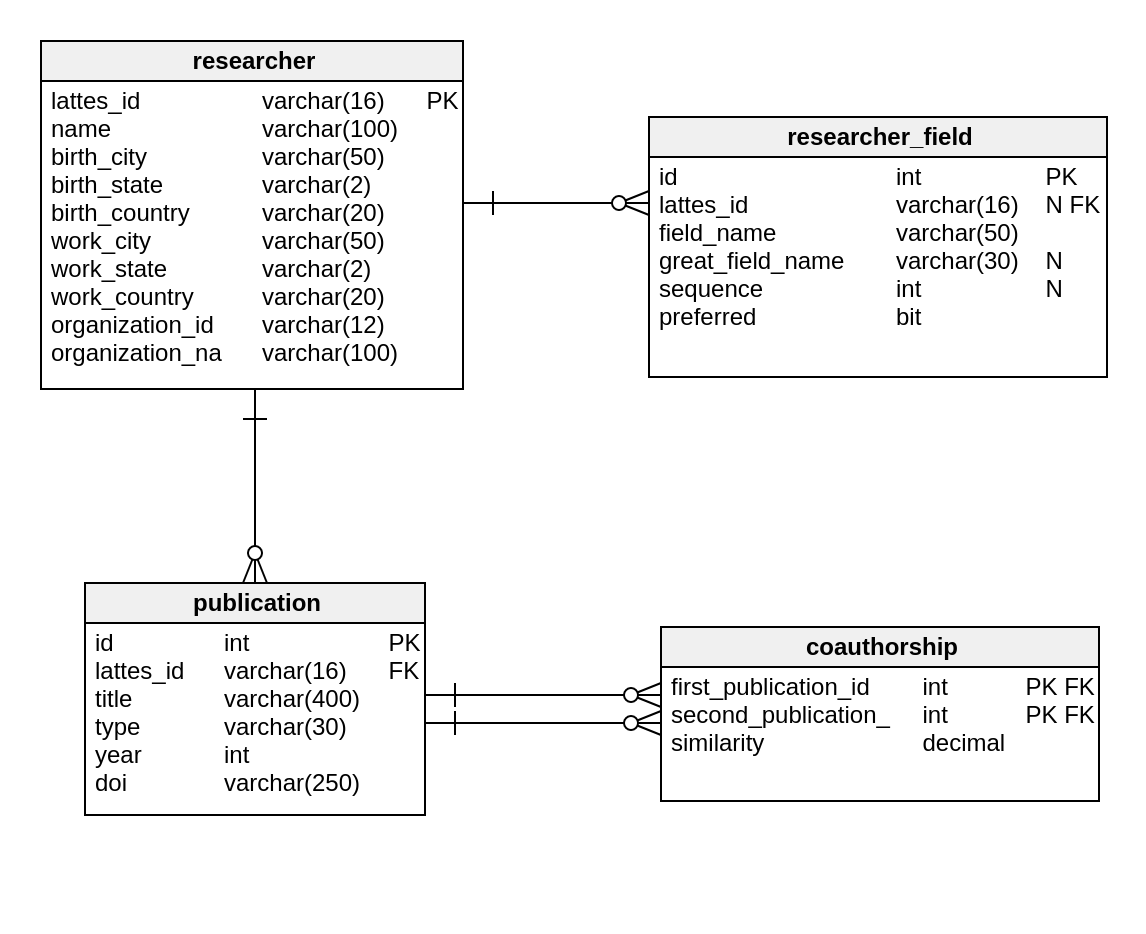
\includegraphics[width=\linewidth, height=\textheight, keepaspectratio]{figuras/apendice-modelo-fisico}
  \caption{Modelo entidade-relacionamento físico do banco de dados construído para armazenar os dados do currículo Lattes.}
  \label{fig:diagramafisico}
\end{figure}

% ----------------------------------------------------------
\chapter{Exemplos de títulos transformados na etapa de pré-processamento do método}
% ----------------------------------------------------------

São apresentados nesta seção alguns exemplos reais de normalização do título que foram feitas pelo \autoref{alg:normalizacao}.

\newcounter{example}[section]
\newenvironment{example}[1][]{\refstepcounter{example}\par\medskip
   \noindent \textbf{Exemplo~\theexample. #1} \rmfamily}{\medskip}

\begin{example}
Título de publicação em inglês inserido dentro de um bloco CDATA
\begin{ABNTEXfontereduzida}
\\ \noindent \textbf{Entrada:}
\begin{verbatim}
    <![CDATA[Multi-Histogram Equalization Methods for Contrast Enhancement and 
    Brightness Preserving]]>
\end{verbatim}

\noindent \textbf{Saída:}
\begin{verbatim}
    multi-histogramequalizationmethodsforcontrastenhancementand
    brightnesspreserving
\end{verbatim}
\end{ABNTEXfontereduzida}
\end{example}

\begin{example}
Título em inglês com letras gregas em codificação HTML
\begin{ABNTEXfontereduzida}
\\ \noindent \textbf{Entrada:}
\begin{verbatim}
    &alpha;-bisabolol-loaded lipid-core nanocapsules reduce lipopolysaccharide-induced 
    pulmonary inflammation in mice
\end{verbatim}

\noindent \textbf{Saída:}
\begin{verbatim}
    α-bisabolol-loadedlipid-corenanocapsulesreducelipopolysaccharide-induced
    pulmonaryinflammationinmice
\end{verbatim}
\end{ABNTEXfontereduzida}
\end{example}

\begin{example}
Título em português com palavras acentuadas
\begin{ABNTEXfontereduzida}
\\ \noindent \textbf{Entrada:}
\begin{verbatim}
    Eidos: a idéia de justiça em Platão
\end{verbatim}

\noindent \textbf{Saída:}
\begin{verbatim}
    eidos:aideiadejusticaemplatao
\end{verbatim}
\end{ABNTEXfontereduzida}
\end{example}


% ----------------------------------------------------------
\chapter{Exemplo de área de atuação inferida para o pesquisador na etapa de pré-processamento do método}
% ----------------------------------------------------------

Nesta seção é apresentado um exemplo construído para demonstrar o resultado produzido pelo \autoref{alg:identificacaoarea} que infere a área de atuação do pesquisador.

\begin{example}
Área de atuação mais presente como Ciência da Informação, mas com prioridade para a Ciência da Computação, dado que pertence a uma grande área com a mesma frequência das outras e aparece listada antes
\begin{ABNTEXfontereduzida}
\\ \noindent \textbf{Entrada:}
\begin{enumerate}
  \item Grande área: Ciências Exatas e da Terra. 
  \item Grande área: Ciências Exatas e da Terra / Área: Ciência da Computação / Subárea: Bibliometria.
  \item Grande área: Ciências Sociais Aplicadas / Área: Ciência da Informação.
  \item Grande área: Ciências Sociais Aplicadas / Área: Ciência da Informação / Subárea: Biblioteconomia.
\end{enumerate}

\noindent \textbf{Saída:}
Área = Ciência da Computação
\end{ABNTEXfontereduzida}
\end{example}

\end{apendicesenv}
% ---